\documentclass{article}

\usepackage[hscale=0.7,vscale=0.8]{geometry}

\usepackage{times}
\usepackage{helvet}
\usepackage{courier}
\usepackage{amsmath,epsfig}
\usepackage{graphicx}
\usepackage{fancyhdr}
\usepackage{times,amsmath,epsfig}
\usepackage{comment}
\usepackage{nccold}
\usepackage{verbatim}
\usepackage[noend]{algorithmic}
\usepackage{color}
\usepackage{url}
\usepackage{float}
\usepackage{alltt}
\usepackage[stable]{footmisc}
\usepackage{subfigure}
\usepackage{epsfig}
\usepackage{amssymb}
\usepackage{amsmath}
\usepackage{amsfonts}
\usepackage{multicol}
\usepackage{caption}
\usepackage{pdflscape}
\usepackage{algorithmic, algorithm}
\usepackage{float}
\usepackage{array}
\usepackage{amsthm}

\DeclareMathOperator*{\argmin}{\arg\!\min}
\DeclareMathOperator*{\argmax}{\arg\!\max}



\def\script#1{\mathcal{#1}}
\def\mS{\script{S}}
\def\mR{\script{R}}

\setlength\parindent{0pt}

\date{}
\title{Discrete Mixture Models}

\author{Trevor Fiez and Jose Picado}

\begin{document}
	\maketitle

\section{Introduction}

Probability mass function for first bonomial:
\begin{align*}
\phi_1(k_1(i)) = p(k_1(i) | p) = \binom{n}{k_1(i)} p^{k_1(i)} (1-p)^{n - k_1(i)}
\end{align*}

Probability mass function for second binomial:
\begin{align*}
\phi_0(k_1(i)) = p(k_1(i) | q) = \binom{n}{k_1(i)} q^{k_1(i)} (1-q)^{n - k_1(i)}
\end{align*}

Probability mass function for mixture model:
\begin{align*}
p(k_1(1), \cdots, k_1(N) | \alpha, p, q) &= \prod_{i=1}^{N} \left[ \alpha \phi_1(k_1(i)) + (1-\alpha)\phi_0(k_1(i)) \right] \\
&= \prod_{i=1}^{N} \left[ \alpha \binom{n}{k_1(i)} p^{k_1(i)} (1-p)^{n - k_1(i)} + (1-\alpha) \binom{n}{k_1(i)} q^{k_1(i)} (1-q)^{n - k_1(i)}  \right]
\end{align*}



\section{FIM and CRLB}

The derivation for the FIM is included in the appendix. Given equation 1 let the loglikihood be

\begin{align*}
\log L(\mathbb{\theta}) &= \sum_{i=1}^{N} \log \left[ \alpha \binom{n}{k_1(i)} p^{k_1(i)} (1-p)^{n - k_1(i)} + (1-\alpha) \binom{n}{k_1(i)} q^{k_1(i)} (1-q)^{n - k_1(i)}  \right] 
\end{align*}

Then it follows that the Fisher Information Matrix and the Cramer-Rao Lower Bound are

\begin{align*}
FIM &= -\mathrm{E} \left[\frac{d^2 \log p}{d^2\mathbb{\theta}}\right] \\
CRLB &= FIM^{-1}
\end{align*}

The derivations for the derivatives are included in the appendix. When doing the derivations we define

\begin{align*}
P(k | p, n) &= \binom{n}{k}p^{k}(1 - p)^{n - k} \\
P'(k | p, n) &= \frac{dP}{dp} = \binom{n}{k}\left[kp^{k - 1}(1 - p)^{n - k} + (n - k)p^{k}(1 - p)^{n - k - 1}\right]\\
P"(k | p, n) &= \frac{d^2P}{d^2p} = \binom{n}{k}\left[k(k - 1)p^{k - 2}(1 - p)^{n - k} + 2k(n - k)p^{k - 1}(1 - p)^{n - k - 1} + (n - k)(n - k - 1)p^k(1 - p)^{n - k - 2}\right]\\
\end{align*}

The Fisher information matrix is then:

\begin{align*}
-E\begin{bmatrix}\frac{\delta^2\log(L(\mathbb{\theta})}{{\delta\theta}^2}\end{bmatrix} &= -N * E\begin{bmatrix}
F_{\alpha\alpha} F_{\alpha p} F_{\alpha q} \\
F_{\alpha p} F_{pp} F_{pq} \\
F_{\alpha q} F_{pq} F_{qq} \\
\end{bmatrix}
\end{align*}

Where

\begin{align*}
F_{\alpha\alpha} &= \frac{\partial^2L(\mathbb{\theta})}{\partial\alpha^2} = \frac{(P(k | p, n) - P(k | q, n))^2}{(\alpha P(k | p, n) + (1 - \alpha) P(k | q, n))^2} \\
F_{\alpha p} &= \frac{\partial^2L(\mathbb{\theta})}{\partial\alpha\partial p} = \frac{P'(k | p, n)P(k | q, n)}{(\alpha P(k | p, n) + (1 - \alpha) P(k | q, n))^2} \\
F_{\alpha q} &= \frac{\partial^2L(\mathbb{\theta})}{\partial\alpha\partial q} = \frac{-P(k | p, n)P'(k | q, n)}{(\alpha P(k | p, n) + (1 - \alpha) P(k | q, n))^2} \\
F_{pp} &= \frac{\partial^2L(\mathbb{\theta})}{\partial p^2} = \frac{\alpha^2P"(k | p, n)P(k | p, n) + \alpha(1 - \alpha)P"(k | p, n)P(k | q, n) - \alpha^2P(k | p, n)^2}{(\alpha P(k | p, n) + (1 - \alpha) P(k | q, n))^2} \\
F_{pq} &= \frac{\partial^2L(\mathbb{\theta})}{\partial p\partial q} = \frac{-\alpha(1 - \alpha)P'(k | p, n)P'(k | p, n)}{(\alpha P(k | p, n) + (1 - \alpha) P(k | q, n))^2} \\
F_{qq} &= \frac{\partial^2L(\mathbb{\theta})}{\partial q^2} = \frac{\alpha(1 - \alpha)P"(k | q, n)P(k | p, n) + (1 - \alpha)^2P"(k | q, n)P(k | q, n) - (1 - \alpha)^2P'(k | q, n)^2}{(\alpha P(k | p, n) + (1 - \alpha) P(k | q, n))^2}
\end{align*}

\section{Maximum Likelihood and Expectation-Maximization}

\subsection{Maximum Likelihood Equations}
Given Equation \ref{main_pmf}, let the likelihood be
\begin{align*}
L(\mathbb{\theta}) = p(k_1(1), \cdots, k_1(N) | \mathbb{\theta})\ 
\end{align*}
Then, the log-likelihood is
\begin{align*}
\log L(\mathbb{\theta}) &= \sum_{i=1}^{N} \log \left[ \alpha \binom{n}{k_1(i)} p^{k_1(i)} (1-p)^{n - k_1(i)} + (1-\alpha) \binom{n}{k_1(i)} q^{k_1(i)} (1-q)^{n - k_1(i)}  \right] 
\end{align*}

The maximum log-likelihood is given by
\begin{align*}
\hat{\theta} = \argmax_{\theta} \log L(\mathbb{\theta})
\end{align*}
Therefore, the maximum likelihood equations are given by:
%Want to do: $\frac{\delta \log p}{\delta \mathbf{\theta}} = \mathbf{0}$

\begin{align*}
\frac{\delta \log p}{\delta \mathbf{\theta}} &= \begin{bmatrix} 
\sum_{i=1}^{N} \frac{\phi_1(k_1(i)) - \phi_0(k_1(i))}{\alpha \phi_1(k_1(i)) + (1-\alpha)\phi_0(k_1(i))} \\ 
\sum_{i=1}^{N} \frac{\alpha \binom{n}{k_1(i)} \left( k_1(i) p^{k_1(i)-1} (1-p)^{n-k_1(i)} - p^{k_1(i)} (n-k_1(i)) (1-p)^{n-k_1(i)-1} \right) }{\alpha \phi_1(k_1(i)) + (1-\alpha)\phi_0(k_1(i))} \\ 
\sum_{i=1}^{N} \frac{(1-\alpha) \binom{n}{k_1(i)} \left( k_1(i) q^{k_1(i)-1} (1-q)^{n-k_1(i)} - q^{k_1(i)} (n-k_1(i)) (1-q)^{n-k_1(i)-1} \right) }{\alpha \phi_1(k_1(i)) + (1-\alpha)\phi_0(k_1(i))} \end{bmatrix} = \mathbf{0}
\end{align*}

\subsection{EM Algorithm}

Let $\mathbf{k_1} = k_1(1), \cdots, k_1(N)$ be the observed data. 
We introduce membership variables $\mathbf{y} = y(i), \cdots, y(N)$ (hidden data) such that $p(y(i) = c) = \alpha_c$. Because we only have two classes, then 
\begin{align*}
p(y(i) = 1) &= \alpha \\
p(y(i) = 0) &= 1-p(y(i) = 1) = 1 - \alpha
\end{align*}

The joint probability mass function is given by:
\begin{align*}
p(\mathbf{k_1}, \mathbf{y} | \theta ) &= \prod_{i=1}^{N} p(k_1(i), y(i) | \theta ) \\
&= \prod_{i=1}^{N} p(k_1(i) | y(i) ) p(y(i) | \theta )  \\
&= \prod_{i=1}^{N} \prod_{l=1}^{M} (\phi_l(k_1(i) \alpha_l)) ^ {I(y(i)=l)}
\end{align*}

Let $Q$ be an auxiliary function such that
\begin{align*}
Q(\theta, \theta') &= \mathrm{E} \left[ \log p(\mathbf{k_1}, \mathbf{y} | \theta ) | \mathbf{k_1}, \theta' \right] \\
&= \mathrm{E} \left[ \sum_{i=1}^{N} \sum_{l=1}^{M} I(y(i)=l) (\log \phi_l(k_1(i)) + \log \alpha_l) | \mathbf{k_1}, \theta' \right] \\
&= \sum_{i=1}^{N} \sum_{l=1}^{M} \mathrm{E} \left[ I(y(i)=l) | \mathbf{k_1}, \theta' \right] (\log \phi_l(k_1(i)) + \log \alpha_l)  \\
&= \sum_{i=1}^{N} \sum_{l=1}^{M} p(y(i) = c | k_1(i), \theta') (\log \phi_l(k_1(i)) + \log \alpha_l)
\end{align*}

In the E-step of the EM algorithm, we compute $p(y(i) = c | k_1(i), \theta')$. 
In our case of $M=2$ the E-step is given by:
\begin{align*}
p(y(i) = 1 | k_1(i), \mathbf{\theta'}) &= \frac{\alpha \binom{n}{k_1(i)} p^{k_1(i)} (1-p)^{n-k_1(i)}}{\alpha \binom{n}{k_1(i)} p^{k_1(i)} (1-p)^{n-k_1(i)} + (1-\alpha) \binom{n}{k_1(i)} q^{k_1(i)} (1-q)^{n-k_1(i)}} \\
p(y(i) = 0 | k_1(i), \mathbf{\theta'}) &= \frac{(1-\alpha) \binom{n}{k_1(i)} q^{k_1(i)} (1-q)^{n-k_1(i)}}{\alpha \binom{n}{k_1(i)} p^{k_1(i)} (1-p)^{n-k_1(i)} + (1-\alpha) \binom{n}{k_1(i)} q^{k_1(i)} (1-q)^{n-k_1(i)}}
\end{align*}

In the M-step, we compute
\begin{align*}
\theta^{k+1} &= \argmax_\theta Q(\theta, \theta^{k}) \\
&= \argmax_\theta \sum_{i=1}^{N} \sum_{l=1}^{M} p(y(i) = l | k_1(i), \theta^{k}) (\log \phi_l(k_1(i)) + \log \alpha_l)
\end{align*}
In our case of $M=2$, we have
\begin{align*}
\theta^{k+1} &= \argmax_\theta \sum_{i=1}^{N} [ p(y(i) = 1 | k_1(i), \theta^{k}) (\log \phi_1(k_1(i)) + \log \alpha) + \\
& \quad \quad \quad \quad \quad \quad \quad p(y(i) = 0 | k_1(i), \theta^{k}) (\log \phi_0(k_1(i)) + \log (1-\alpha)) ]
\end{align*}

We first maximize $\alpha$. Using Lagrangiang, we get
\begin{align*}
L &= \sum_{i=1}^{N} \sum_{l=1}^{M} p(y(i) = c | k_1(i), \theta^{k}) (\log \alpha_l) + \lambda(\sum_{l=1}^{M} \alpha_l - 1)
\end{align*}
Then, taking the derivative
\begin{align*}
\frac{\delta L}{\delta \alpha} &= \sum_{i=1}^{N} \sum_{l=1}^{M} p(y(i) = c | k_1(i), \theta^{k}) \frac{1}{\alpha_l} + \lambda &= 0
\alpha_l &= -\frac{1}{\lambda} 
\end{align*}


To maximize $p$, we get:
\begin{align*}
p^{k+1} &= \argmax_p \sum_{i=1}^{N}  p(y(i) = 1 | k_1(i), \theta^{k}) \log \phi_1(k_1(i)) \\
&= \argmax_p \sum_{i=1}^{N}  p(y(i) = 1 | k_1(i), \theta^{k}) \log \binom{n}{k_1(i)} p^{k_1(i)} (1-p)^{n-k_1(i)}  \\
&= \argmax_p \sum_{i=1}^{N}  p(y(i) = 1 | k_1(i), \theta^{k}) (\log n! - \log k_1(i)! - \log (n-k_1(i))! + k_1(i) \log p + (n-k_1(i)) \log (1-p))
\end{align*}
Taking the derivative and making equal to 0:
\begin{align*}
\frac{\delta}{\delta p} &= \sum_{i=1}^{N}  p(y(i) = 1 | k_1(i), \theta^{k}) \left( \frac{k_1(i)}{p} + \frac{n-k_1(i)}{1-p} \right) \\
&= \sum_{i=1}^{N}  p(y(i) = 1 | k_1(i), \theta^{k}) \left( \frac{k_1(i)(1-p) - (n-k_1(i))p}{p(1-p)}
\right) \\
&= \sum_{i=1}^{N}  p(y(i) = 1 | k_1(i), \theta^{k}) \left( \frac{k_1(i)- k_1(i)p - np +k_1(i)p}{p(1-p)} \right) \\
&= \sum_{i=1}^{N}  p(y(i) = 1 | k_1(i), \theta^{k}) \left( \frac{k_1(i)- np}{p(1-p)} \right) \\
&= \frac{1}{p(1-p)} \sum_{i=1}^{N} p(y(i) = 1 | k_1(i), \theta^{k}) k_1(i) - \frac{1}{p(1-p)} \sum_{i=1}^{N} p(y(i) = 1 | k_1(i), \theta^{k}) np \\
&= 0 \\
\end{align*}
Therefore, the value that maximizes $p$ is
\begin{align*}
p^{k+1} = \frac{\sum_{i=1}^{N} p(y(i) = 1 | k_1(i), \theta^{k}) k_1(i)}{n \sum_{i=1}^{N} p(y(i) = 1 | k_1(i), \theta^{k})}
\end{align*}
To maximize $q$, we take a similar derivation from the one taken for $p$. Therefore, the value that maximizes $q$ is
\begin{align*}
q^{k+1} &= \frac{\sum_{i=1}^{N} p(y(i) = 0 | k_1(i), \theta^{k}) k_1(i)}{n \sum_{i=1}^{N} p(y(i) = 0 | k_1(i), \theta^{k})}
\end{align*}


Then, we get:
\begin{align*}
\alpha_1^{k+1} &= \alpha^{k+1} = \frac{1}{N} \sum_{i=1}^{N} p(y(i) = 1 | k_1(i), \theta^{k}) \\
\alpha_0^{k+1} &= 1 - \alpha^{k+1} \\
p^{k+1} &= \frac{\sum_{i=1}^{N} p(y(i) = 1 | k_1(i), \theta^{k}) k_1(i)}{n \sum_{i=1}^{N} p(y(i) = 1 | k_1(i), \theta^{k})} \\
q^{k+1} &= \frac{\sum_{i=1}^{N} p(y(i) = 0 | k_1(i), \theta^{k}) k_1(i)}{n \sum_{i=1}^{N} p(y(i) = 0 | k_1(i), \theta^{k})}
\end{align*}


\begin{figure}[!htbp]
	\centering
	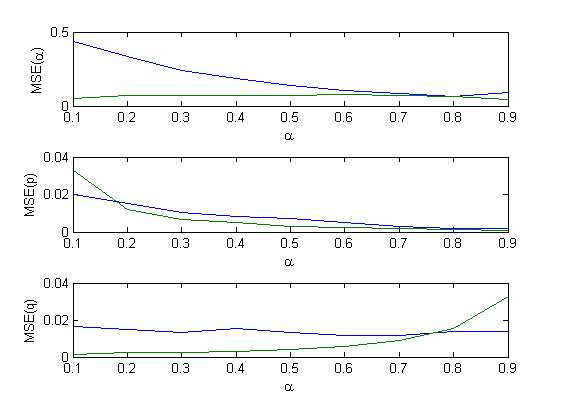
\includegraphics[width=\columnwidth]{images/EM_plot.png} %height=1.7in,
	\vspace{-1pt}
	\caption{CRLB (green) vs EM (blue).}
	\vspace{-2pt}
	\label{figure:crlb-em}
\end{figure}


\section{Method of Moments}

\section{Experiments}

We used the Expectation-Maximization (EM) estimator and Method of Moments (MOM) estimator to estimate the parameters of the discrete mixture of models described in Section \ref{introduction}. We compare the estimators with the CRLB derived in Section 2.

The parameters in our model are $\alpha$, $p$, and $q$. We generated data using fixed values for these parameters, and then ran the estimators to find the values for these parameters. 
We applied the process for $p=0.2$, $q=0.4$, and for $\alpha=0.1, 0.2, \cdots, 0.9$. 
We set the length of each sequence to be $n=20$, and generated $N=200$ i.i.d. sequences.
We ran 200 independent Monte-Carlo runs.
We ran the EM algorithm for 100 iterations.

We compare the mean squared error (MSE) of each estimator and compare it to the CRLB.
The results are shown in Figure \ref{figure:crlb-em-mom}. 
As can be seen, the estimators have a bigger MSE when $\alpha=0.1$ or $\alpha=0.9$. 
This is because with $\alpha=0.1$, the data generator obtained sequences from the distribution $P(k_i(i)|p,n)$ with small probability.
The same happens when $\alpha=0.9$, where the data generator obtained sequences from the distribution $P(k_i(i)|q,n)$ with small probability.
The higher the probability that the data generator obtained sequences from a distribution, the easier it is for the estimators to estimate the correct value.
The performance of EM and MOM estimators is very similar, with differences mainly with small and large values for $\alpha$.

As can be seen, the CRLB is very low, compared to both estimators. 
To visualize the difference more clearly, we plotted the same results with a log-scale on the $y$ axis. 
The results are shown in Figure \ref{figure:crlb-em-mom-logscale}.
As can be seen, the CRLB is always more than 2 orders of magnitude lower than the results obtained by the estimators. 
We believe this is because the CRLB is not a tight bound. 
Therefore, in this case, the results obtained by the estimators do not get close to the CRLB.

\begin{figure}[!htbp]
	\centering
	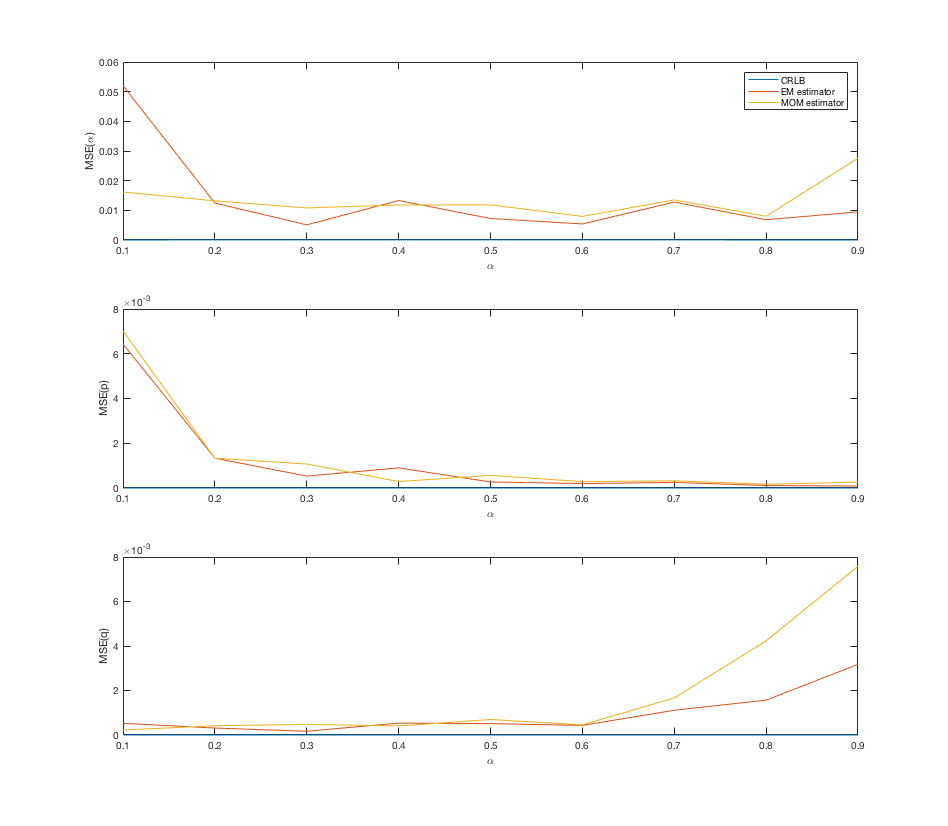
\includegraphics[width=\columnwidth]{images/CRLB_EM_MOM.png}
	\caption{CRLB, EM and MOM results for estimating $\alpha$ (top), $p$, (middle) and $q$ (bottom).}
	\label{figure:crlb-em-mom}
\end{figure}

\begin{figure}[!htbp]
	\centering
	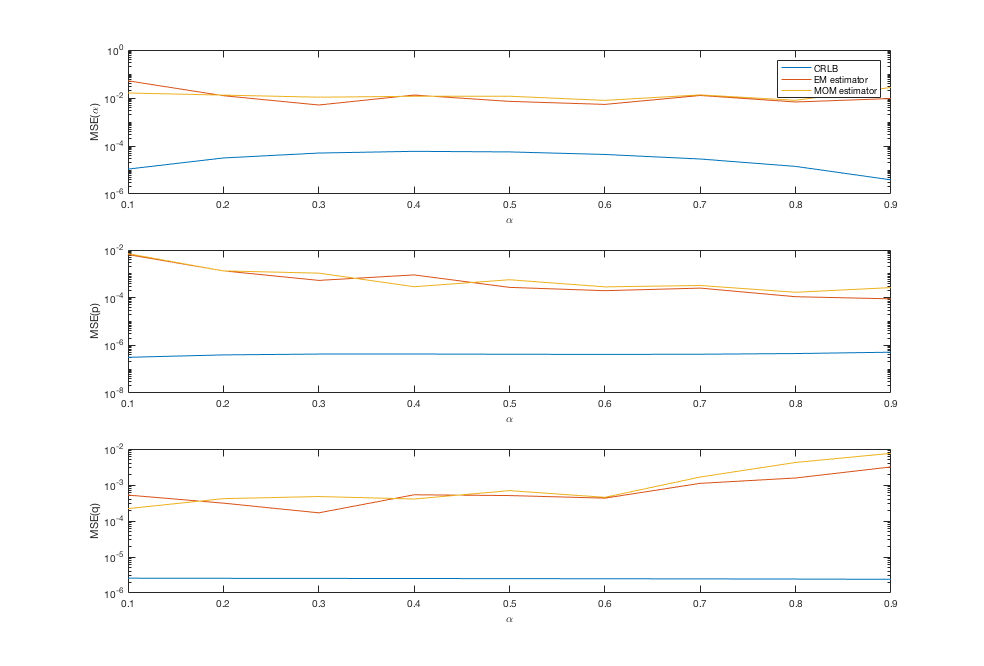
\includegraphics[width=\columnwidth]{images/CRLB_EM_MOM_log.png}
	\caption{CRLB, EM and MOM results for estimating $\alpha$ (top), $p$, (middle) and $q$ (bottom) with log-scale on the $y$ axis.}
	\label{figure:crlb-em-mom-logscale}
\end{figure}

\subsection{EM Initialization}

The performance of the EM algorithm may be affected by the initialization of the parameters. 
To evaluate the impact of initialization, we experimented with three methods of initialization.
The first method consists in setting initial values by selecting a random value from a uniform distribution between 0 and 1. This is the easiest method. However, the estimator may get stuck in a local minima.
In the second method, we use K-means clustering \cite{DBLP:journals/corr/BlomerB13}. This is a more informed method of initialization, without requiring much computational cost.
For the third method, we set the initial values to be the exact values that we used to generate the data. Although this is not reasonable in a practical sense, we consider this to be an ``empirical lower bound".
The results of running the EM algorithm with the described initialization methods are shown in Figure \ref{figure:em-init}. 
As can be seen, random initialization performs worse when $\alpha$ is low. 
However, it reaches a similar performance as other initialization methods with greater values of $\alpha$. 
K-Means initialization helps the estimator to obtain a lower MSE and get closer to our empirical lower bound.


\begin{figure}[!htbp]
	\centering
	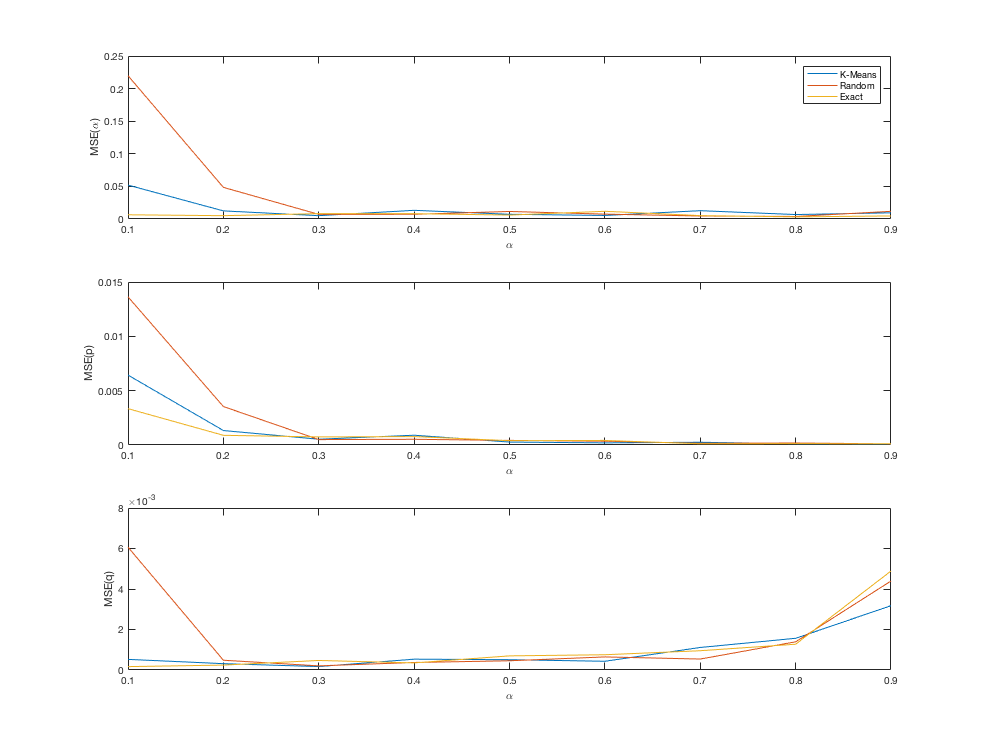
\includegraphics[width=\columnwidth]{images/compare_EM_init.png}
	\caption{EM results with different initializations for estimating $\alpha$ (top), $p$, (middle) and $q$ (bottom).}
	\label{figure:em-init}
\end{figure}


\section{Conclusion}


We derived the FIM and CRLB for estimating the parameters of a mixture model of two binomial distributions with $M=2$ different categories. 
Our derivations can easily be extended to multimodal distributions with any number of categories.
We showed the Maximum Likelihood equations for our problem.
Because the equations do not have a closed-form solution, we used the EM algorithm to obtain an esimator. We derived the equations needed to perform the E-step and M-step.
We also showed how to use a MOM estimator, where we simply use the first, second, and third order moments to generate a system of equations. By solving this system, we obtain the estimates for our parameters.
We showed in the empirical results that CRLB is a very low bound, as EM and MOM do not get close to it.
EM and MOM estimators have a similar performance, with differences only in the edge cases.
We also showed the impact of initialization on the EM algorithm. 

\bibliographystyle{abbrv}
\bibliography{ref}

\appendix
\section{Derivations}

As a reminder here are the equations for P

\begin{align*}
P(k | p, n) &= \binom{n}{k}p^{k}(1 - p)^{n - k} \\
P'(k | p, n) &= \frac{dP}{dp} = \binom{n}{k}\left[kp^{k - 1}(1 - p)^{n - k} + (n - k)p^{k}(1 - p)^{n - k - 1}\right]\\
P''(k | p, n) &= \frac{d^2P}{dp^2} = \binom{n}{k}\left[k(k - 1)p^{k - 2}(1 - p)^{n - k} - (-k + n - 1)(n - k)p^k(1 - p)^{-k + n - 2} \right]\\
\end{align*}

Deriving derivatives for the FIM beginning with the first derivative of L($\theta$)

\begin{align*}
\frac{\delta \log L}{\delta \mathbf{\theta}} &= N \begin{bmatrix} 
 \frac{P(k | p, n) - P(k | q, n)}{\alpha P(k | p, n) + (1-\alpha)P(k | q, n)} \\ 
\frac{\alpha P'(k | p, n)}{\alpha P(k | p, n) + (1-\alpha)P(k | q, n)} \\ 
\frac{(1 - \alpha) P'(k | q, n)}{\alpha P(k | p, n) + (1-\alpha)P(k | q, n)} \\  \end{bmatrix}
\end{align*}

The second derivatives were derived as follows

\begin{align*}
F_{\alpha\alpha} &= \frac{\partial^2\log P(\mathbb{\theta})}{\partial\alpha^2} \\
F_{\alpha\alpha} &= \frac{\partial}{\partial\alpha}\frac{P(k | p, n) - P(k | q, n)}{\alpha P(k | p, n) + (1-\alpha)P(k | q, n)} \\
F_{\alpha\alpha} &= \frac{-(P(k | p, n) - P(k | q, n))^2}{(\alpha P(k | p, n) + (1 - \alpha) P(k | q, n))^2} \\
\end{align*}

\begin{align*}
F_{\alpha p} &= \frac{\partial^2\log L(\mathbb{\theta})}{\partial\alpha\partial p} \\
F_{\alpha p} &= \frac{\partial}{\partial p}\frac{P(k | p, n) - P(k | q, n)}{\alpha P(k | p, n) + (1-\alpha)P(k | q, n)} \\
F_{\alpha p} &= \frac{P'(k | p, n)}{\alpha P(k | p, n) + (1-\alpha)P(k | q, n)} - \frac{(P(k | p, n) - P(k | q, n))\alpha P'(k | p, n)}{(\alpha P(k | p, n) + (1 - \alpha) P(k | q, n))^2} \\
F_{\alpha p} &= \frac{\alpha P'(k | p, n)P(k | p. n) + (1 - \alpha)P(k | p, n)P(k | q, n) - \alpha P'(k | p, n)P(k | p, n) + \alpha P'(k | p, n)P(k | q, n)}{(\alpha P(k | p, n) + (1 - \alpha) P(k | q, n))^2} \\
F_{\alpha p} &= \frac{P'(k | p, n)P(k | q, n)}{(\alpha P(k | p, n) + (1 - \alpha) P(k | q, n))^2}
\end{align*}

\begin{align*}
F_{\alpha q} &= \frac{\partial^2\log L(\mathbb{\theta})}{\partial\alpha\partial q} \\
F_{\alpha q} &= \frac{\partial}{\partial q}\frac{P(k | p, n) - P(k | q, n)}{\alpha P(k | p, n) + (1-\alpha)P(k | q, n)} \\
F_{\alpha q} &= \frac{-P'(k | q, n)}{\alpha P(k | p, n) + (1-\alpha)P(k | q, n)} - \frac{(P(k | p, n) - P(k | q, n))(1 - \alpha)P'(k | q, n)}{(\alpha P(k | p, n) + (1 - \alpha) P(k | q, n))^2} \\
F_{\alpha q} &= \frac{-\alpha P'(k | q, n)P(k | p, n) - (1 - \alpha)P'(k | q, n)P(k | q, n) - (1 - \alpha)P'(k | q, n)P(k | p, n) + (1 - \alpha)P'(k | q, n)P(k | q, n)}{(\alpha P(k | p, n) + (1 - \alpha) P(k | q, n))^2} \\
F_{\alpha q} &= \frac{-P'(k | q, n)P(k | p, n)}{(\alpha P(k | p, n) + (1 - \alpha) P(k | q, n))^2}
\end{align*}

\begin{align*}
F_{pp} &= \frac{\partial^2\log L(\mathbb{\theta})}{\partial p^2} \\
F_{pp} &= \frac{\partial}{\partial p}\frac{\alpha P'(k | p, n)}{\alpha P(k | p, n) + (1-\alpha)P(k | q, n)} \\ 
F_{pp} &= \frac{\alpha P''(k | p, n)}{\alpha P(k | p, n) + (1-\alpha)P(k | q, n)} - \frac{(\alpha P'(k, | p, n))^2)}{(\alpha P(k | p, n) + (1 - \alpha) P(k | q, n))^2} \\
F_{pp} &= \frac{\alpha^2P''(k | p, n)P(k | p, n) + \alpha(1 - \alpha)P''(k | p, n)P(k | q, n) - \alpha^2P'(k | p, n)^2}{(\alpha P(k | p, n) + (1 - \alpha) P(k | q, n))^2} \\
\end{align*}

\begin{align*}
F_{pq} &= \frac{\partial^2\log L(\mathbb{\theta})}{\partial p\partial q} \\
F_{pq} &= \frac{\partial}{\partial q}\frac{\alpha P'(k | p, n)}{\alpha P(k | p, n) + (1-\alpha)P(k | q, n)} \\ 
F_{pq} &= \frac{-\alpha(1 - \alpha)P'(k | p, n)P'(k | q, n)}{(\alpha P(k | p, n) + (1 - \alpha) P(k | q, n))^2} \\
\end{align*}

\begin{align*}
F_{qq} &= \frac{\partial^2\log L(\mathbb{\theta})}{\partial q^2} \\
F_{qq} &= \frac{\partial}{\partial q}\frac{(1 - \alpha) P'(k | q, n)}{\alpha P(k | p, n) + (1-\alpha)P(k | q, n)} \\
F_{qq} &= \frac{(1 - \alpha) P''(k | q, n)}{\alpha P(k | p, n) + (1-\alpha)P(k | q, n)} - \frac{((1 - \alpha)P'(k | q, n))^2}{(\alpha P(k | p, n) + (1 - \alpha) P(k | q, n))^2} \\
F_{qq} &= \frac{\alpha(1 - \alpha)P''(k | q, n)P(k | p, n) + (1 - \alpha)^2P''(k | q, n)P(k | q, n) - (1 - \alpha)^2P''(k | q, n)^2}{(\alpha P(k | p, n) + (1 - \alpha) P(k | q, n))^2}
\end{align*}



\end{document}

